\chapter{Theory of Unconstrained Optimization}
\label{chap:unconstrained}

%%%%%%%%%%%%%%%%%%%%%%%%%%%%%%%%%%%%%%%%%%%%%%%%%%%%%%%%%%%%
\section{Introduction}
\label{sec:2.1}

%%%%%%%%%%%%%%%%%%%%%%%%%%%%%%%%%%%%%%%%%%%%%%%%%%%%%%%%%%%%
\subsection{General Problem}
\label{subsec:2.1.1}

We consider the unconstrained optimization problem
\begin{equation}
    \min_{x \in \mathbb{R}^n} f(x),
\end{equation}
where $n \geq 1$ and $f : \mathbb{R}^n \to \mathbb{R}$ is assumed to be sufficiently smooth
(typically $\mathcal{C}^1$ or $\mathcal{C}^2$).

\begin{remarque}
We leave aside nonsmooth optimization: it can be difficult to analyze the
local behavior of $f$ in the neighborhood of $x_k$. For a general presentation,
see for example Hiriart-Urruty and Lemaréchal.
\end{remarque}

%%%%%%%%%%%%%%%%%%%%%%%%%%%%%%%%%%%%%%%%%%%%%%%%%%%%%%%%%%%%
\subsection{Reformulation}
\label{subsec:2.1.2}

It is sometimes possible to reformulate a nonsmooth problem into a smooth problem
by increasing the dimension.

Let $f_1,\dots,f_m : \mathbb{R}^n \to \mathbb{R}$ be smooth functions, and define
\begin{equation}
    f(x) = \max_{j=1,\dots,m} f_j(x).
\end{equation}
Then the problem
\begin{equation}
    (P) :\quad \min_{x \in \mathbb{R}^n} f(x)
        = \min_{x \in \mathbb{R}^n} \max_{1 \le j \le m} f_j(x)
\end{equation}
is a nonsmooth problem constructed from smooth functions.

This problem can be rewritten as
\begin{equation}
    \min_{(x,t)\in\mathbb{R}^{n+1}} t
    \quad \text{under the constraints } \quad
    t - f_j(x) \ge 0,\quad j=1,\dots,m,
\end{equation}
the latter condition meaning
\begin{equation}
    f_j(x) \le t,\quad j=1,\dots,m.
\end{equation}

\begin{figure}[H]
\centering
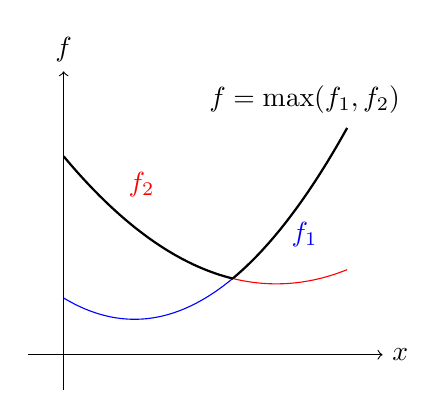
\begin{tikzpicture}[scale=0.9]
    \draw[->] (-0.5,0) -- (4.5,0) node[right] {$x$};
    \draw[->] (0,-0.5) -- (0,4) node[above] {$f$};
    % f1
    \draw[domain=0:4,smooth,variable=\x,blue]
        plot ({\x},{0.3*(\x-1)^2+0.5});
    \node[blue] at (3.4,1.7) {$f_1$};
    % f2
    \draw[domain=0:4,smooth,variable=\x,red]
        plot ({\x},{0.2*(\x-3)^2+1});
    \node[red] at (1.1,2.4) {$f_2$};
    % max = upper envelope: f2 before intersection (x≈2.39), f1 after
    \draw[domain=0:2.39,smooth,variable=\x,thick]
        plot ({\x},{0.2*(\x-3)^2+1});
    \draw[domain=2.39:4,smooth,variable=\x,thick]
        plot ({\x},{0.3*(\x-1)^2+0.5});
    \node[thick] at (3.4,3.6) {$f = \max(f_1,f_2)$};
\end{tikzpicture}
\caption{Example of a nonsmooth function $f(x)=\max(f_1(x),f_2(x))$.}
\label{fig:max_func}
\end{figure}

\begin{figureexplanation}
In Figure~\ref{fig:max_func}, the thick black curve represents the function $f(x) = \max(f_1(x), f_2(x))$. It follows the upper portion of each curve: $f_2$ (red) when $x$ is small, and $f_1$ (blue) when $x$ is large. The intersection point marks a break in the slope, making $f$ non-differentiable at this point (nonsmooth function).
\end{figureexplanation}

%%%%%%%%%%%%%%%%%%%%%%%%%%%%%%%%%%%%%%%%%%%%%%%%%%%%%%%%%%%%
\section{Identifying Minimizers}
\label{sec:2.2}

%%%%%%%%%%%%%%%%%%%%%%%%%%%%%%%%%%%%%%%%%%%%%%%%%%%%%%%%%%%%
\subsection*{Definitions}
\label{subsec:2.2.0}

\begin{definition}
Let $f : \mathbb{R}^n \to \mathbb{R}$. A point $x^\star \in \mathbb{R}^n$ is
\begin{itemize}
    \item a \textbf{global minimizer} of $f$ if
    \[
        f(x^\star) \leq f(x), \quad \forall x \in \mathbb{R}^n ;
    \]
    \item a \textbf{local minimizer (weak)} if there exists a neighborhood $V$ of $x^\star$
    such that
    \[
        f(x^\star) \leq f(x), \quad \forall x \in V ;
    \]
    \item a \textbf{strict local minimizer} if there exists a neighborhood $V$ of $x^\star$
    such that
    \[
        f(x^\star) < f(x), \quad \forall x \in V \setminus \{x^\star\} ;
    \]
    \item an \textbf{isolated local minimizer} if there exists a neighborhood $V$ of $x^\star$
    such that $x^\star$ is the unique local minimizer of $f$ in $V$.
\end{itemize}
\end{definition}

%%%%%%%%%%%%%%%%%%%%%%%%%%%%%%%%%%%%%%%%%%%%%%%%%%%%%%%%%%%%
\subsection{Taylor's Theorem}
\label{subsec:2.2.1}

\begin{theoreme}[Mean Value Theorem]
\label{thm:MVT}
Suppose that $f : \mathbb{R}^n \to \mathbb{R}$ is continuously differentiable ($\mathcal{C}^1$).
Then for all $x \in \mathbb{R}^n$ and all $\eta \in \mathbb{R}^n$, there exists
$t \in (0,1)$ such that
\begin{equation}
    f(x+\eta) = f(x) + \nabla f(x+t\eta)^\top \eta.
\end{equation}
\end{theoreme}



\begin{theoreme}[Taylor Expansions]
\label{thm:Taylor}
If $f : \mathbb{R}^n \to \mathbb{R}$ is twice continuously differentiable ($\mathcal{C}^2$), then for all
$x,\eta \in \mathbb{R}^n$:
\begin{enumerate}
    \item There exists $t_1 \in (0,1)$ such that
    \[
        \nabla f(x + \eta) = \nabla f(x) + \nabla^2 f(x + t_1\eta)\,\eta.
    \]
    \item There exists $t_2 \in (0,1)$ such that
    \[
        f(x + \eta) = f(x) + \nabla f(x)^\top \eta + \tfrac{1}{2}\,\eta^\top \nabla^2 f(x + t_2\eta)\,\eta.
    \]
\end{enumerate}
\end{theoreme}

\paragraph{Gradient and Hessian.}

For $f : \mathbb{R}^n \to \mathbb{R}$, the gradient at $x$ is
\[
\nabla f(x) =
\begin{pmatrix}
\displaystyle \frac{\partial f}{\partial x_1}(x)\\[0.3em]
\vdots\\[0.3em]
\displaystyle \frac{\partial f}{\partial x_n}(x)
\end{pmatrix}
\in \mathbb{R}^n.
\]

The Hessian matrix of $f$ at $x \in \mathbb{R}^n$ is
\[
\nabla^2 f(x) =
\begin{pmatrix}
\frac{\partial^2 f}{\partial x_1^2}(x) &
\cdots &
\frac{\partial^2 f}{\partial x_1 \partial x_n}(x)\\
\vdots & \ddots & \vdots \\
\frac{\partial^2 f}{\partial x_n \partial x_1}(x) &
\cdots &
\frac{\partial^2 f}{\partial x_n^2}(x)
\end{pmatrix}
\in \mathbb{R}^{n \times n}.
\]

For $x \in \mathbb{R}^n$, we also denote $x^\top = (x_1,\dots,x_n)$.

%%%%%%%%%%%%%%%%%%%%%%%%%%%%%%%%%%%%%%%%%%%%%%%%%%%%%%%%%%%%
\subsection{First-Order Necessary Condition}
\label{subsec:2.2.2}

\begin{theoreme}[First-Order Necessary Condition]
\label{thm:first-order}
Suppose that $f$ is continuously differentiable in a neighborhood of $x^\star$, and
that $x^\star$ is a local minimizer of $f$. Then
\begin{equation}
    \nabla f(x^\star) = 0.
\end{equation}
\end{theoreme}

\begin{proof}
We reason by contradiction. Suppose that $\nabla f(x^\star) \neq 0$ and let
$\eta = -\nabla f(x^\star) \neq 0$. Since $f$ is $\mathcal{C}^1$ in the neighborhood of
$x^\star$, we have
\[
    \eta^\top \nabla f(x^\star) = -\|\nabla f(x^\star)\|^2 < 0.
\]
By the mean value theorem, there exists $t \in (0,T)$ such that
\[
    f(x^\star + t\eta) = f(x^\star) + t\,\nabla f(x^\star + t'\eta)^\top \eta
\]
for some $t' \in (0,t)$. For $t>0$ small enough, the product
$\nabla f(x^\star + t'\eta)^\top \eta$ remains strictly negative by continuity.
We then obtain
\[
    f(x^\star + t\eta) < f(x^\star),
\]
and this holds for all $t \in [0,T]$: we have indeed captured a descent direction, and not just an isolated point. This contradicts the fact that $x^\star$ is a local minimizer. Thus, we must have
$\nabla f(x^\star) = 0$.
\end{proof}

%%%%%%%%%%%%%%%%%%%%%%%%%%%%%%%%%%%%%%%%%%%%%%%%%%%%%%%%%%%%
\subsection{Second-Order Necessary Condition}
\label{subsec:2.2.3}

\begin{definition}
A point $x^\star$ is a \emph{stationary point} of $f$ if
\[
    \nabla f(x^\star) = 0.
\]
Theorem \ref{thm:first-order} states that every local minimizer is a stationary point.
\end{definition}

\begin{theoreme}[Second-Order Necessary Condition]
\label{thm:second-order-necessary}
Suppose that $f$ is twice continuously differentiable in a neighborhood of $x^\star$,
and that $x^\star$ is a local minimizer of $f$. Then
\[
    \nabla f(x^\star) = 0
    \quad\text{and}\quad
    \nabla^2 f(x^\star) \succeq 0,
\]
that is
\[
    \forall \eta \in \mathbb{R}^n,\quad
    \eta^\top \nabla^2 f(x^\star)\,\eta \ge 0.
\]
\end{theoreme}

\begin{proof}
We already know by \autoref{thm:first-order} that $\nabla f(x^\star)=0$.
Let us reason by contradiction for the Hessian. Suppose that $\nabla^2 f(x^\star)$
is not positive semi-definite. Then there exists $\eta \in \mathbb{R}^n$
such that
\[
    \eta^\top \nabla^2 f(x^\star)\,\eta < 0.
\]
By continuity of $\nabla^2 f$ in the neighborhood of $x^\star$, there exists $T>0$ such that
\[
    \forall t \in [0,T],\quad
    \eta^\top \nabla^2 f(x^\star + t\eta)\,\eta < 0.
\]
In particular, for $t\in(0,T)$, the Taylor expansion gives
\[
    f(x^\star + t\eta)
    = f(x^\star) + t\,\nabla f(x^\star)^\top \eta
      + \frac{t^2}{2}\,\eta^\top \nabla^2 f(x^\star + \theta t\eta)\,\eta
\]
for some $\theta \in (0,1)$. Since $\nabla f(x^\star)=0$ and
$\eta^\top \nabla^2 f(x^\star + \theta t\eta)\,\eta < 0$, we obtain
\[
    f(x^\star + t\eta) < f(x^\star),
\]
and this for all $t \in [0,T]$: we have a descent direction and not an isolated point. This contradicts the fact that $x^\star$ is a local minimizer.
Therefore, $\nabla^2 f(x^\star)$ must be positive semi-definite.
\end{proof}

%%%%%%%%%%%%%%%%%%%%%%%%%%%%%%%%%%%%%%%%%%%%%%%%%%%%%%%%%%%%
\subsection{Second-Order Sufficient Condition}
\label{subsec:2.2.4}

\begin{theoreme}[Second-Order Sufficient Condition]
\label{thm:second-order-sufficient}
Suppose that $f$ is twice continuously differentiable on an open neighborhood of $x^\star$,
and that
\[
    \nabla f(x^\star) = 0,\qquad
    \nabla^2 f(x^\star) \succ 0,
\]
that is
\[
    \forall \eta \in \mathbb{R}^n\setminus\{0\},\quad
    \eta^\top \nabla^2 f(x^\star)\,\eta > 0.
\]
Then $x^\star$ is a strict local minimizer of $f$.
\end{theoreme}

\begin{proof}
The Hessian is continuous and positive definite at $x^\star$. There thus exists $r>0$ such that
$\nabla^2 f(x) \succ 0$ for all $x$ in the ball
\[
    D = \{ x \in \mathbb{R}^n \;|\; \|x - x^\star\| < r \}.
\]
Let $\eta \in \mathbb{R}^n$ such that $\|\eta\| \le r$.
By Taylor's theorem \ref{thm:Taylor}, there exists $t \in (0,1)$ such that
\[
    f(x^\star + \eta)
    = f(x^\star)
      + \eta^\top \nabla f(x^\star)
      + \tfrac{1}{2}\,\eta^\top \nabla^2 f(x^\star + t\eta)\,\eta.
\]
Since $\nabla f(x^\star) = 0$ and $\nabla^2 f(x^\star + t\eta) \succ 0$, we deduce
\[
    f(x^\star + \eta) > f(x^\star)
\]
as soon as $\eta \neq 0$ and $\|\eta\|$ is small enough. Thus $x^\star$ is a
strict local minimizer.
\end{proof}

%%%%%%%%%%%%%%%%%%%%%%%%%%%%%%%%%%%%%%%%%%%%%%%%%%%%%%%%%%%%
\subsection{Convex Case}
\label{subsec:2.2.5}

\begin{theoreme}[Convex Case]
\label{thm:convex-case}
Let $f : \mathbb{R}^n \to \mathbb{R}$ be a convex function.
\begin{enumerate}
    \item Every local minimizer of $f$ is also a global minimizer.
    \item If $f$ is additionally differentiable, then every stationary point
    ($\nabla f(x^\star) = 0$) is a global minimizer.
\end{enumerate}
\end{theoreme}

\begin{proof}[Proof of point (1)]
Suppose that $x^\star$ is a local minimizer but not a global one. Then there exists
$y \in \mathbb{R}^n$ such that
\[
    f(y) < f(x^\star).
\]
By convexity of $f$, for all $\lambda \in [0,1]$ we have
\[
    f(\lambda x^\star + (1-\lambda)y)
    \le \lambda f(x^\star) + (1-\lambda) f(y) < f(x^\star) \qquad (\lambda \neq 1).
\]
Let $V$ be a neighborhood of $x^\star$. For $\lambda \in (0,1)$ sufficiently small,
the point $z = \lambda x^\star + (1-\lambda)y$ belongs to $V$ and satisfies
$f(z) < f(x^\star)$, which contradicts the local minimality of $x^\star$.
\end{proof}

%%%%%%%%%%%%%%%%%%%%%%%%%%%%%%%%%%%%%%%%%%%%%%%%%%%%%%%%%%%%
\section{Iteration Strategies}
\label{sec:2.3}

Optimization algorithms build a sequence $(x_k)_{k\ge 0}$ such that
\[
    x_{k+1} = x_k + \alpha_k p_k,
\]
where $p_k$ is a search direction (generally a descent direction) and $\alpha_k > 0$
is a step length (displacement length).

In practice:
\begin{itemize}
    \item we choose a starting point $x_0$,
    \item at iteration $k$, we use local information (values of $f$, of
    $\nabla f$, or even $\nabla^2 f$) to define $p_k$ and $\alpha_k$,
    \item we typically seek to ensure
    \[
        f(x_{k+1}) < f(x_k),
    \]
    or at least a decrease after several iterations:
    \[
        f(x_{k+m}) < f(x_k).
    \]
\end{itemize}

Two large families of strategies exist:
\begin{itemize}
    \item \textbf{trust region} methods,
    \item \textbf{line search} methods.
\end{itemize}

%%%%%%%%%%%%%%%%%%%%%%%%%%%%%%%%%%%%%%%%%%%%%%%%%%%%%%%%%%%%
\subsection{Trust Region Methods}
\label{subsec:2.3.1}

At iteration $k$, we fix a radius $\Delta_k > 0$ defining the trust region
around $x_k$:
\[
    \{x \in \mathbb{R}^n \;|\; \|x - x_k\| \le \Delta_k\}.
\]

Using Taylor's formula, we approximate $f$ by a quadratic model
\begin{equation}
    m_k(x) = f(x_k) + (x-x_k)^\top \nabla f(x_k)
             + \tfrac{1}{2}(x-x_k)^\top \nabla^2 f(x_k)\,(x-x_k).
\end{equation}
We then choose $x_{k+1}$ as a solution (or an approximation of the solution)
of the trust region problem
\begin{equation}
    x_{k+1} = \arg\min_{x} \; m_k(x)
    \quad \text{s.t. } \|x - x_k\| \le \Delta_k.
\end{equation}
Letting $p_k = x_{k+1} - x_k$, this amounts to minimizing $m_k(p)$ under the
constraint $\|p\| \le \Delta_k$:
\begin{equation}
    p_k = \arg\min_{\|p\| \le \Delta_k}
    \Big( f(x_k) + \nabla f(x_k)^\top p
          + \tfrac{1}{2}p^\top \nabla^2 f(x_k)\,p \Big).
\end{equation}

We introduce the ratio
\begin{equation}
    \rho_k =
    \frac{f(x_k) - f(x_k + p_k)}{m_k(0) - m_k(p_k)}.
\end{equation}
The typical acceptance rules are:
\begin{itemize}
    \item if $\rho_k < 0$: the new iteration is rejected, and we reduce $\Delta_k$;
    \item if $0 < \rho_k$ is small: we accept $x_{k+1}$ but keep $\Delta_k$
    roughly unchanged;
    \item if $\rho_k \approx 1$: we accept $x_{k+1}$ and increase $\Delta_k$.
\end{itemize}

%%%%%%%%%%%%%%%%%%%%%%%%%%%%%%%%%%%%%%%%%%%%%%%%%%%%%%%%%%%%
\subsection{Line Search Methods}
\label{subsec:2.3.2}

Line search methods take the form
\[
    x_{k+1} = x_k + \alpha_k p_k,
\]
where $p_k$ is a descent direction and $\alpha_k$ is adaptively chosen step length.

A frequent choice for the direction $p_k$ is
\begin{equation}
    p_k = -B_k \nabla f_k,
\end{equation}
where $B_k$ is a symmetric positive definite (or at least invertible) matrix and
\[
    f_k = f(x_k),\quad \nabla f_k = \nabla f(x_k),\quad
    \nabla^2 f_k = \nabla^2 f(x_k).
\]
In this case, we have
\begin{equation}
    p_k^\top \nabla f_k
    = -\nabla f_k^\top B_k \nabla f_k < 0,
\end{equation}
since $B_k$ is positive definite and $\nabla f_k \neq 0$. Thus $p_k$ is
indeed a descent direction. Furthermore
\[
    p_k^\top \nabla f_k
    = \|p_k\|\,\|\nabla f_k\|\cos(\angle(p_k,\nabla f_k)) < 0,
\]
which implies that the angle between $p_k$ and $\nabla f_k$ is strictly greater
than $\frac{\pi}{2}$.

\medskip

The basic idea is to choose $\alpha_k$ as
\[
    \alpha_k = \arg\min_{\alpha>0} \varphi(\alpha),
    \qquad \varphi(\alpha) = f(x_k + \alpha p_k),
\]
but this one-dimensional problem can be expensive to solve exactly. We
therefore search for an \emph{acceptable} value $\alpha_k$, satisfying sufficient
decrease conditions.

\paragraph{Sufficient decrease condition (Armijo).}

We impose
\begin{equation}
\label{eq:Armijo}
    f(x_k + \alpha p_k)
    \le f(x_k) + c_1\,\alpha\,\nabla f_k^\top p_k,
\end{equation}
where $c_1 \in (0,1)$ is a parameter (typically $c_1 = 10^{-4}$).

\begin{figure}[H]
\centering
\begin{tikzpicture}[scale=1.0]
    \draw[->] (0,0) -- (5,0) node[right] {$\alpha$};
    \draw[->] (0,-0.5) -- (0,4) node[above] {$\varphi(\alpha)$};

    % reference point
    \fill (0,3) circle (1pt);
    \node[left] at (0,3) {$\varphi(0)$};

    % decreasing curve
    \draw[domain=0:4,smooth,variable=\x,thick]
        plot ({\x},{3 - 1.5*\x + 0.3*\x*\x});

    % Armijo line
    \draw[domain=0:4,smooth,variable=\x,dashed]
        plot ({\x},{3 - 0.8*\x});

    \node[right] at (4.2, -0.5) {$\varphi(0) + c_1\alpha \varphi'(0)$};

\end{tikzpicture}
\caption{Sufficient decrease condition (Armijo).}
\label{fig:armijo}
\end{figure}

\begin{figureexplanation}
Figure~\ref{fig:armijo} illustrates the sufficient decrease condition: the curve of the function $\varphi(\alpha)$ must lie below the dotted line with equation $\varphi(0) + c_1 \alpha \varphi'(0)$. This guarantees that the function decreases sufficiently relative to its initial slope.
\end{figureexplanation}

\begin{remarque}
The Armijo condition is always satisfied for sufficiently small $\alpha$.
It ensures that the decrease of $f$ is proportional to $\alpha$ and to the
directional derivative $\nabla f_k^\top p_k$.
\end{remarque}
\begin{definition}[Wolfe Conditions]
We say that $\alpha$ satisfies the \emph{Wolfe conditions} if
\begin{align}
    f(x_k + \alpha p_k)
    &\le f(x_k) + c_1 \alpha \nabla f_k^\top p_k, \\
    \nabla f(x_k + \alpha p_k)^\top p_k
    &\ge c_2 \nabla f_k^\top p_k,
\end{align}
for constants $0 < c_1 < c_2 < 1$.
By denoting $\varphi(\alpha) = f(x_k + \alpha p_k)$, the second condition
can also be written as $\varphi'(\alpha) \ge c_2 \varphi'(0)$.
\end{definition}

\begin{definition}[Strong Wolfe Conditions]
The \emph{strong Wolfe conditions} are obtained by replacing the
previous curvature condition by
\begin{equation}
    |\nabla f(x_k + \alpha p_k)^\top p_k|
    \le -c_2 \nabla f_k^\top p_k,
\end{equation}
that is
\[
    |\varphi'(\alpha)| \le -c_2 \varphi'(0).
\]
This excludes values of $\alpha$ for which the slope is too positive.
\end{definition}

\begin{remarque}[Comparison standard vs strong Wolfe]
    The strong Wolfe condition reinforces the standard condition with an upper and lower bound.
    \begin{itemize}
        \item \textbf{Standard Wolfe: } $\varphi'(\alpha) \ge c_2 \varphi'(0)$. It forbids slopes that are too negative, but allows very positive slopes (overshooting the minimum).
        \item \textbf{Strong Wolfe: } $|\varphi'(\alpha)| \le -c_2 \varphi'(0) \iff c_2 \varphi'(0) \le \varphi'(\alpha) \le -c_2 \varphi'(0)$. It also forbids slopes that are too positive, forcing $\alpha$ to stay in a neighborhood where the derivative is close to zero.
    \end{itemize}
\end{remarque}

\begin{figure}[H]
\centering
\begin{tikzpicture}[scale=1.0]
    % Axes
    \draw[->] (0,0) -- (6,0) node[right] {$\alpha$};
    \draw[->] (0,-0.5) -- (0,4) node[above] {$\varphi(\alpha)$};
    
    % Reference point
    \fill (0,3) circle (1.5pt);
    \node[left] at (0,3) {$\varphi(0)$};
    
    % phi(alpha) curve - decreasing then increasing
    \draw[domain=0:5, smooth, variable=\x, thick, blue]
        plot ({\x},{3 - 1.8*\x + 0.35*\x*\x});
    \node[blue, right] at (5, 2.95) {$\varphi(\alpha)$};
    
    % Armijo line (sufficient decrease)
    \draw[domain=0:5, smooth, variable=\x, dashed, red]
        plot ({\x},{3 - 0.5*\x});
    \node[red, right] at (5, 0.5) {$\varphi(0) + c_1\alpha\varphi'(0)$};
    
    % Curvature condition: phi'(alpha) >= c2 * phi'(0)
    % Acceptable zone bounds roughly at 1.8 and 3.71
    
    \fill[green!25, opacity=0.6] 
        (1.8, {3 - 0.5*1.8}) --
        (3.71, {3 - 0.5*3.71}) --
        plot[domain=3.71:1.8, smooth, variable=\x] ({\x},{3 - 1.8*\x + 0.35*\x*\x}) --
        cycle;
    
    \draw[<->, thick, green!60!black] (1.8, -0.3) -- (3.71, -0.3);
    \node[below, green!60!black] at (2.75, -0.3) {\small acceptable (Wolfe)};
    
    \draw[dotted, green!60!black] (1.8, 0) -- (1.8, {3 - 0.5*1.8});
    \draw[dotted, green!60!black] (3.71, 0) -- (3.71, {3 - 0.5*3.71});
    
    \coordinate (curvPt) at (1.8, 0.894);
    \draw[-, thick, orange] ($(curvPt) + (-0.5, 0.27)$) -- ($(curvPt) + (0.7, -0.378)$);
    \filldraw[orange] (curvPt) circle (2pt);
    \node[orange, left] at (0.8, 0.6) {\small $\varphi'(\alpha) = c_2\varphi'(0)$};
\end{tikzpicture}
\caption{Wolfe conditions: the acceptable zone (green) satisfies both the sufficient decrease (Armijo) and the curvature condition.}
\label{fig:wolfe-complete}
\end{figure}

\begin{figureexplanation}
In Figure~\ref{fig:wolfe-complete}, the \textbf{acceptable zone} (in green) is the interval of steps $\alpha$ which simultaneously satisfy the two Wolfe conditions:
1. The Armijo condition (sufficient decrease): the blue curve is below the red line.
2. The curvature condition: the slope of the curve (orange tangent) is greater than or equal to $c_2$ times the initial slope.
\end{figureexplanation}

\begin{remarque}
For methods of the Newton or quasi-Newton type, one often chooses
$c_2 \approx 0.9$, while for nonlinear conjugate gradient methods,
one tends to take $c_2 \approx 0.1$.
\end{remarque}

\begin{lemme}
\label{lem:Wolfe-existence}
Suppose that $f$ is continuously differentiable ($\mathcal{C}^1$) and that $p_k$ is a descent
direction. Suppose that $f$ is bounded from below along the ray
\[
    \{ x_k + \alpha p_k \;|\; \alpha > 0 \}.
\]
Then, for any $0 < c_1 < c_2 < 1$, there exist intervals of values of
$\alpha$ satisfying the Wolfe conditions (standard or strong).
\end{lemme}

\begin{proof}
Let $\varphi(\alpha) = f(x_k + \alpha p_k)$, and $\varphi'(0) = \nabla f_k^\top p_k < 0$.
Since $f$ is bounded from below on the ray, $\varphi$ is as well.

For $c_1 \in (0,1)$, consider the affine function
\[
    \ell(\alpha) = f(x_k) + c_1 \alpha \nabla f_k^\top p_k.
\]
Since $\ell(\alpha) \to -\infty$ as $\alpha \to +\infty$, the graphs of
$\varphi$ and $\ell$ intersect. Let $\hat{\alpha}>0$ be the smallest intersection
point:
\[
    \varphi(\hat{\alpha})
    = f(x_k + \hat{\alpha} p_k)
    = f(x_k) + c_1 \hat{\alpha}\,\nabla f_k^\top p_k.
\]
The Armijo condition is therefore strictly verified for all $\alpha \in (0,\hat{\alpha})$.

By the mean value theorem, there exists $\bar{\alpha} \in (0,\hat{\alpha})$ such that
\[
    \varphi(\hat{\alpha}) - \varphi(0)
    = \hat{\alpha}\,\varphi'(\bar{\alpha}).
\]
Combining with the definition of $\hat{\alpha}$, we obtain
\[
    c_1 \nabla f_k^\top p_k
    = \varphi'(\bar{\alpha}).
\]
Since $c_1 < c_2$ and $\nabla f_k^\top p_k < 0$, it comes
\[
    c_2 \nabla f_k^\top p_k < \varphi'(\bar{\alpha}),
\]
which is the Wolfe condition
\[
    \nabla f(x_k + \bar{\alpha} p_k)^\top p_k > c_2 \nabla f_k^\top p_k.
\]
By continuity of $\varphi'$ and $\varphi$, this condition and the Armijo
condition remain valid in a small interval around $\bar{\alpha}$, which
gives an interval of $\alpha$ satisfying the Wolfe conditions. Moreover,
since $\varphi'(\bar{\alpha})<0$, we can also satisfy the strong Wolfe
condition on a neighboring interval.
\end{proof}

\paragraph{Line search by \emph{backtracking}.}

A simple way to ensure the Armijo condition is the \emph{backtracking line search}.

\begin{algorithm}[H]
\caption{Line search with backtracking}
\label{alg:backtracking}
Choose $\bar{\alpha} > 0$, $\rho \in (0,1)$, $c \in (0,1)$; Set $\alpha \leftarrow \bar{\alpha}$\;
\Repeat{$f(x_k + \alpha p_k) \le f(x_k) + c\alpha\nabla f_k^\top p_k$}{
    $\alpha \leftarrow \rho\alpha$\;
}
Terminate with $\alpha_k = \alpha$.
\end{algorithm}

\begin{remarque}
In practice, we almost always start the line search with $\bar{\alpha} = 1$.
\end{remarque}

\paragraph{Line search algorithm with zoom.}

To satisfy the Wolfe conditions, a more sophisticated algorithm that uses a \emph{zoom} procedure is used.

\begin{algorithm}[H]
\caption{Line search algorithm}
\label{alg:line-search}
Set $\alpha_0 \leftarrow 0$, choose $\alpha_{\max} > 0$ and $\alpha_1 \in (0, \alpha_{\max})$\;
$i \leftarrow 1$\;
\Repeat{}{
    Evaluate $\phi(\alpha_i)$\;
    \If{$\phi(\alpha_i) > \phi(0) + c_1\alpha_i\phi'(0)$ \Or $[\phi(\alpha_i) \ge \phi(\alpha_{i-1})$ \And $i > 1]$}{
        $\alpha_* \leftarrow \texttt{zoom}(\alpha_{i-1}, \alpha_i)$ \And \Stop\;
    }
    Evaluate $\phi'(\alpha_i)$\;
    \If{$|\phi'(\alpha_i)| \le -c_2\phi'(0)$}{
        set $\alpha_* \leftarrow \alpha_i$ \And \Stop\;
    }
    \If{$\phi'(\alpha_i) \ge 0$}{
        set $\alpha_* \leftarrow \texttt{zoom}(\alpha_i, \alpha_{i-1})$ \And \Stop\;
    }
    Choose $\alpha_{i+1} \in (\alpha_i, \alpha_{\max})$\;
    $i \leftarrow i + 1$\;
}
\end{algorithm}

\begin{algorithm}[H]
\caption{Zoom procedure}
\label{alg:zoom}
\Repeat{}{
    Interpolate to find a trial step length $\alpha_j$ between $\alpha_{lo}$ and $\alpha_{hi}$\;
    Evaluate $\phi(\alpha_j)$\;
    \If{$\phi(\alpha_j) > \phi(0) + c_1\alpha_j\phi'(0)$ \Or $\phi(\alpha_j) \ge \phi(\alpha_{lo})$}{
        $\alpha_{hi} \leftarrow \alpha_j$\;
    }
    \Else{
        Evaluate $\phi'(\alpha_j)$\;
        \If{$|\phi'(\alpha_j)| \le -c_2\phi'(0)$}{
            Set $\alpha_* \leftarrow \alpha_j$ \And \Stop\;
        }
        \If{$\phi'(\alpha_j)(\alpha_{hi} - \alpha_{lo}) \ge 0$}{
            $\alpha_{hi} \leftarrow \alpha_{lo}$\;
        }
        $\alpha_{lo} \leftarrow \alpha_j$\;
    }
}
\end{algorithm}

\begin{remarque}
The function $\phi(\alpha) = f(x_k + \alpha p_k)$ and $\phi'(\alpha) = \nabla f(x_k + \alpha p_k)^\top p_k$.
The constants $c_1$ and $c_2$ are those of the Wolfe conditions, with typically $c_1 = 10^{-4}$ and $c_2 = 0.9$.
\end{remarque}

%%%%%%%%%%%%%%%%%%%%%%%%%%%%%%%%%%%%%%%%%%%%%%%%%%%%%%%%%%%%
\section{Search Directions for Line Search}
\label{sec:2.4}

%%%%%%%%%%%%%%%%%%%%%%%%%%%%%%%%%%%%%%%%%%%%%%%%%%%%%%%%%%%%
\subsection{Gradient Descent (steepest descent)}
\label{subsec:2.4.1}

Let $p$ be a direction and $\alpha>0$ a step. The Taylor expansion gives
\[
    f(x_k + \alpha p)
    = f(x_k) + \alpha\,p^\top \nabla f(x_k)
      + \frac{\alpha^2}{2}\,p^\top \nabla^2 f(x_k + t p)\,p
\]
for some $t \in (0,\alpha)$. The linear rate of change of $f$ along
$p$ is the coefficient of $\alpha$:
\[
    p^\top \nabla f(x_k).
\]

The direction of steepest decrease (of norm $1$) is obtained by solving
\[
    \min_{\|p\|=1} p^\top \nabla f(x_k).
\]
By using
\[
    p^\top \nabla f(x_k)
    = \|p\|\,\|\nabla f(x_k)\|
      \cos(\angle(p,\nabla f(x_k)))
    = \|\nabla f(x_k)\|
      \cos(\angle(p,\nabla f(x_k))),
\]
we see that this minimum is reached when
$\cos(\angle(p,\nabla f(x_k))) = -1$, that is to say when
\[
    p = -\frac{\nabla f(x_k)}{\|\nabla f(x_k)\|}.
\]
The direction of steepest descent is therefore
\begin{equation}
    p_k = -\frac{\nabla f_k}{\|\nabla f_k\|}.
\end{equation}
It is orthogonal to the level curves of $f$ and points in the direction of
maximum instantaneous decrease.

\begin{figure}[H]
\centering
\begin{tikzpicture}[scale=1.0]
    % Level curves (ellipses)
    \draw (0,0) ellipse (2cm and 1.2cm);
    \draw (0,0) ellipse (1.2cm and 0.72cm);
    
    % Optimal point x*
    \filldraw (0,0) circle (1.5pt) node[below] {$x^\star$};
    
    % Point x_k on outer ellipse (2, 1.2)
    \coordinate (xk) at (1.88, -0.41);
    \filldraw (xk) circle (2pt) node[above right] {$x_k$};
    
    % Tangent to the ellipse at point x_k
    \draw[dashed, gray] ($(xk) + (-0.5, -0.85)$) -- ($(xk) + (0.5, 0.85)$);
    
    % Gradient ∇f_k
    \draw[->, thick, blue] (xk) -- +(0.65, -0.39) node[right] {$\nabla f_k$};
    
    % Steepest descent p_k = -∇f_k
    \draw[->, thick, red] (xk) -- +(-0.65, 0.39) node[above left] {$p_k$};
\end{tikzpicture}
\caption{Steepest descent direction.}
\label{fig:steepest-descent}
\end{figure}

\begin{figureexplanation}
Figure~\ref{fig:steepest-descent} shows that the gradient $\nabla f_k$ is orthogonal (perpendicular) to the level curve of $f$ passing through $x_k$ and points outwards (growth of the function). The steepest descent direction $p_k = -\nabla f_k$ is thus also orthogonal to the level curve, but points inwards (maximum local decrease).
\end{figureexplanation}

\begin{remarque}
For gradient descent:
\begin{itemize}
    \item we only require the gradient $\nabla f$;
    \item the direction is always a descent direction:
    \[
        p_k^\top \nabla f_k
        = -\frac{1}{\|\nabla f_k\|}\|\nabla f_k\|^2 < 0 ;
    \]
    \item the method can nevertheless be very slow, particularly on
    poorly conditioned problems.
\end{itemize}
\end{remarque}

\begin{figure}[H]
\centering

\includegraphics[width=0.7\textwidth]{3.png}
\caption{Iterations of the steepest descent method on the level curves of the Rosenbrock function.}
\label{fig:steepest-descent-rosenbrock}
\end{figure}

\begin{figureexplanation}
\textbf{Key points to observe:}
\begin{itemize}
    \item \textbf{Zigzag trajectory:} The method oscillates perpendicularly to the valley, because the gradient always points orthogonally to the level curves.
    \item \textbf{Slow convergence:} Despite multiple iterations, the progress towards the minimum $(1,1)$ is very slow along the valley.
    \item \textbf{Fundamental limitation:} Without curvature information (Hessian), the method cannot "straighten" its direction towards the bottom of the valley.
\end{itemize}
This slow convergence motivates the use of more sophisticated methods (Newton, BFGS, conjugate gradient).
\end{figureexplanation}
%%%%%%%%%%%%%%%%%%%%%%%%%%%%%%%%%%%%%%%%%%%%%%%%%%%%%%%%%%%%
\subsection{Newton Direction}
\label{subsec:2.4.2}

Consider the second-order Taylor approximation
\[
    f(x_k + \eta)
    = f(x_k) + \eta^\top \nabla f(x_k)
      + \tfrac{1}{2}\,\eta^\top \nabla^2 f(x_k + t\eta)\,\eta,
\]
for some $t \in (0,1)$. We approximate $f$ by the quadratic model
\[
    m_k(\eta)
    = f(x_k) + \eta^\top \nabla f(x_k)
      + \tfrac{1}{2}\,\eta^\top \nabla^2 f(x_k)\,\eta.
\]
If the Hessian $\nabla^2 f_k$ is positive definite, minimizing $m_k$ with respect to $\eta$
leads to the optimality condition
\[
    \nabla f_k + \nabla^2 f_k\,\eta_k^N = 0,
\]
i.e.,
\begin{equation}
    \eta_k^N = -(\nabla^2 f_k)^{-1} \nabla f_k.
\end{equation}
The Newton direction is therefore $p_k^N = \eta_k^N$.

If $\nabla^2 f_k \succ 0$, we have
\[
    \nabla f_k^\top p_k^N
    = - (p_k^N)^\top \nabla^2 f_k\, p_k^N < 0,
\]
hence $p_k^N$ is a descent direction.

Moreover, if $\nabla^2 f$ is sufficiently smooth, the error of the Taylor
approximation is of order
\[
    f(x_k + \eta) - m_k(\eta) = \mathcal{O}(\|\eta\|^3).
\]

\begin{remarque}
The natural step in Newton's method is $\alpha = 1$:
\[
    x_{k+1} = x_k + p_k^N = x_k - (\nabla^2 f_k)^{-1}\nabla f_k.
\]
In practice, a line search is often performed (e.g., with Wolfe
conditions), starting with $\alpha=1$.
\end{remarque}

%%%%%%%%%%%%%%%%%%%%%%%%%%%%%%%%%%%%%%%%%%%%%%%%%%%%%%%%%%%%
\subsection{Characterization of Convergence}
\label{subsec:2.4.3}

Consider a line search type algorithm
\[
    x_{k+1} = x_k + \alpha_k p_k,
\]
where $p_k$ is a descent direction and $\alpha_k$ satisfies the Wolfe conditions.

\begin{theoreme}[Zoutendijk]
\label{thm:Zoutendijk}
Suppose that:
\begin{itemize}
    \item $f : \mathbb{R}^n \to \mathbb{R}$ is bounded below,
    \item $f$ is continuously differentiable ($\mathcal{C}^1$) on an open set $N \subset \mathbb{R}^n$
    containing the level set
    \[
        \{ x \in \mathbb{R}^n \;|\; f(x) \le f(x_0)\},
    \]
    \item the gradient $\nabla f$ is Lipschitz continuous on $N$, i.e., there exists $L>0$ such that
    \[
        \|\nabla f(x) - \nabla f(y)\| \le L \|x-y\|,
        \quad \forall x,y \in N.
    \]
\end{itemize}
Then
\begin{equation}
    \sum_{k=0}^{\infty} \cos^2(\theta_k)\,\|\nabla f_k\|^2 < +\infty,
\end{equation}
where $\theta_k$ is the angle between $-\nabla f_k$ and the direction $p_k$, defined by
\[
    \cos(\theta_k)
    = \frac{-\nabla f_k^\top p_k}{\|\nabla f_k\|\,\|p_k\|}.
\]
\end{theoreme}

\begin{remarque}
A proof can be found in \cite{nocedal2006numerical}.
\end{remarque}

\paragraph{Illustration 1.}
As a consequence, we obtain
\[
    \cos^2(\theta_k)\,\|\nabla f_k\|^2 \xrightarrow[k\to\infty]{} 0.
\]
If we assume that there exists $\delta>0$ such that
\[
    \cos(\theta_k) \ge \delta > 0, \quad \forall k,
\]
then necessarily
\[
    \|\nabla f_k\| \xrightarrow[k\to\infty]{} 0.
\]

\begin{definition}
An algorithm is said to be \emph{globally convergent} if it satisfies
\[
    \|\nabla f_k\| \to 0
\]
for any sequence of iterates $(x_k)$ generated from a given starting point $x_0$.
In the absence of information about the Hessian, this is the best global result
one can hope for: it guarantees convergence to a \emph{stationary point},
not necessarily a minimizer.
\end{definition}

\paragraph{Illustration 2: Newton's Case.}

Recall the Newton direction
\[
    d_k = \eta_k^N = -(\nabla^2 f_k)^{-1}\nabla f_k,
\]
assuming $\nabla^2 f_k \succ 0$. Suppose that the condition number of the
Hessian is uniformly bounded, i.e., there exists $M>0$ such that
\[
    \|\nabla^2 f_k\|\cdot\|(\nabla^2 f_k)^{-1}\| \le M, \quad \forall k.
\]
Then it can be shown that $\cos(\theta_k)$ is uniformly bounded below
by a strictly positive constant.

Indeed,
\[
    \cos(\theta_k)
    = \frac{-\nabla f_k^\top d_k}{\|\nabla f_k\|\,\|d_k\|}
    = \frac{\nabla f_k^\top (\nabla^2 f_k)^{-1} \nabla f_k}
           {\|\nabla f_k\|\;\|(\nabla^2 f_k)^{-1}\nabla f_k\|}.
\]
We have
\[
    \|(\nabla^2 f_k)^{-1}\nabla f_k\|
    \le \|(\nabla^2 f_k)^{-1}\|\;\|\nabla f_k\|.
\]
Hence
\[
    \cos(\theta_k)
    \ge \frac{\nabla f_k^\top (\nabla^2 f_k)^{-1} \nabla f_k}
              {\|\nabla f_k\|^2 \,\|(\nabla^2 f_k)^{-1}\|}.
\]
Using the Cholesky decomposition $\nabla^2 f_k = LL^\top$,
we get
\[
    \nabla f_k^\top (\nabla^2 f_k)^{-1} \nabla f_k
    = \|L^{-1}\nabla f_k\|^2
    \ge \frac{\|\nabla f_k\|^2}{\|L\|^2}.
\]
Furthermore, for the spectral norm, $\|L\|^2 = \|\nabla^2 f_k\|$.
We then deduce
\[
    \cos(\theta_k)
    \ge \frac{1}{\|\nabla^2 f_k\|\,\|(\nabla^2 f_k)^{-1}\|}
    \ge \frac{1}{M} > 0.
\]
By Zoutendijk's theorem, we conclude that $\|\nabla f_k\| \to 0$.

\begin{remarque}
For certain algorithms, one only proves that
\[
    \liminf_{k\to\infty} \|\nabla f_k\| = 0,
\]
which means that at least one subsequence of iterates converges to a
stationary point.
\end{remarque}

%%%%%%%%%%%%%%%%%%%%%%%%%%%%%%%%%%%%%%%%%%%%%%%%%%%%%%%%%%%%
\subsection{Convergence Rate of Steepest Descent}
\label{subsec:2.4.4}

\paragraph{Quadratic case.}

Consider
\[
    f(x) = \tfrac{1}{2} x^\top Q x - b^\top x,
\]
where $Q$ is symmetric and positive definite.

\begin{theoreme}[Luenberger]
\label{thm:Luenberger}
Let $(x_k)$ be the sequence generated by the steepest descent method (gradient) with
exact line search applied to $f$. Then
\[
    \|x_{k+1} - x^\star\|_Q
    \le \left( \frac{\lambda_{\max} - \lambda_{\min}}
                    {\lambda_{\max} + \lambda_{\min}} \right)
       \|x_k - x^\star\|_Q,
\]
where $x^\star$ is the minimizer of $f$, $\|x\|_Q = \sqrt{x^\top Q x}$, and
$\lambda_{\min} \le \cdots \le \lambda_{\max}$ are the eigenvalues of $Q$.
\end{theoreme}

\begin{exemple}
If $Q = \lambda I$ for some $\lambda>0$, then
\[
    \frac{\lambda_{\max} - \lambda_{\min}}
         {\lambda_{\max} + \lambda_{\min}} = 0,
\]
and convergence occurs in a single iteration.
\end{exemple}

\begin{figure}[H]
    \centering
    % Figure (a) - Equal eigenvalues
    \begin{subfigure}[b]{\textwidth}
        \centering
        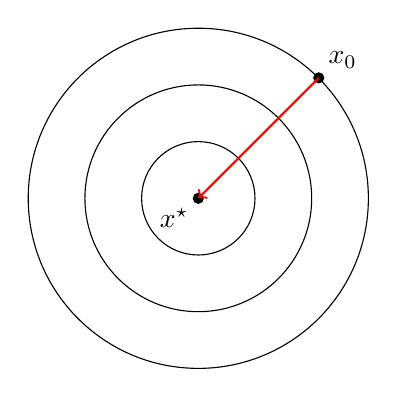
\begin{tikzpicture}[scale=0.9]
            \draw (0,0) circle (0.8cm);
            \draw (0,0) circle (1.6cm);
            \draw (0,0) circle (2.4cm);
            \filldraw (0,0) circle (2pt) node[below left] {$x^\star$};
            \coordinate (x0) at (1.7, 1.7);
            \filldraw (x0) circle (2pt) node[above right] {$x_0$};
            \draw[->, thick, red] (x0) -- (0,0);
        \end{tikzpicture}
        \caption{Equal eigenvalues ($Q=\lambda I$): direct convergence in one iteration.}
    \end{subfigure}
    
    \vspace{0.8cm}
    
    % Figure (b) - Different eigenvalues
    \begin{subfigure}[b]{\textwidth}
        \centering
        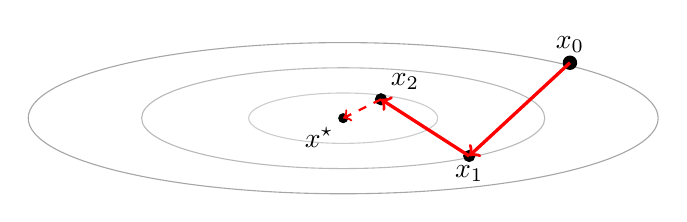
\begin{tikzpicture}[scale=0.8]
            % 3 elongated horizontal ellipses (poor conditioning κ >> 1)
            \draw[gray!70] (0,0) ellipse (5cm and 1.2cm);
            \draw[gray!55] (0,0) ellipse (3.2cm and 0.8cm);
            \draw[gray!40] (0,0) ellipse (1.5cm and 0.4cm);
            
            % Optimal point at the center
            \filldraw (0,0) circle (2pt) node[below left] {$x^\star$};
            
            % Trajectory with clear zigzag (3 arrows)
            \coordinate (x0) at (3.6, 0.88);
            \coordinate (x1) at (2.0, -0.6);
            \coordinate (x2) at (0.6, 0.3);
            
            % Points with labels
            \filldraw (x0) circle (3pt) node[above] {$x_0$};
            \filldraw (x1) circle (2.5pt) node[below] {$x_1$};
            \filldraw (x2) circle (2.5pt) node[above right] {$x_2$};
            
            % Zigzag arrows
            \draw[->, very thick, red] (x0) -- (x1);
            \draw[->, very thick, red] (x1) -- (x2);
            \draw[->, thick, red, dashed] (x2) -- (0,0);
        \end{tikzpicture}
        \caption{Very different eigenvalues ($\kappa \gg 1$): slow zigzag convergence.}
    \end{subfigure}
    \caption{Effect of the conditioning of $Q$ on steepest descent.}
\end{figure}

\textbf{Nonlinear case:}
\begin{theoreme}
\label{thm:SD-nonlinear-rate}
Suppose that $f$ is twice differentiable and that the iterates generated by the
steepest descent method converge to a point $x^\star$ such that the Hessian
$\nabla^2 f(x^\star)$ is positive definite. Let
$\lambda_1 \le \cdots \le \lambda_m$ be the eigenvalues of $\nabla^2 f(x^\star)$
and let
\[
    \omega \in \left(\frac{\lambda_m - \lambda_1}{\lambda_m + \lambda_1}, 1\right).
\]
Then, for $k$ large enough,
\[
    f(x_{k+1}) - f(x^\star)
    \le \omega^2 \bigl( f(x_k) - f(x^\star) \bigr).
\]
\end{theoreme}

\begin{exemple}
Suppose that
\[
    f(x_0) = 1, \qquad f(x^\star) = 0,
\]
and that
\[
    \kappa\bigl(\nabla^2 f(x^\star)\bigr)
    = \|\nabla^2 f(x^\star)\|\;\bigl\|\bigl(\nabla^2 f(x^\star)\bigr)^{-1}\bigr\|
    = \frac{\lambda_m}{\lambda_1} = 800.
\]
Then the linear convergence constant is
\[
    \omega = \frac{800 - 1}{800 + 1}.
\]
After $1000$ iterations,
\[
    f(x_{1001}) \approx \omega^{2000} f(x_0) \approx 0.082.
\]
\end{exemple}

\begin{definition}[Rate of convergence]
\label{def:convergence-rates}
Let $(x_k)$ be a sequence converging to $x^\star$.
\begin{itemize}
    \item We say that $(x_k)$ converges \emph{Q-linearly} to $x^\star$ if there exists
    $\omega \in (0,1)$ and $k_0$ such that
    \[
        \frac{\|x_{k+1} - x^\star\|}{\|x_k - x^\star\|}
        \le \omega, \quad \forall k \ge k_0.
    \]
    \item The convergence is \emph{Q-superlinear} if
    \[
        \frac{\|x_{k+1} - x^\star\|}{\|x_k - x^\star\|}
        \xrightarrow[k\to\infty]{} 0.
    \]
    \item The convergence is \emph{Q-quadratic} if there exists $M>0$ and $k_0$ such that
    \[
        \frac{\|x_{k+1} - x^\star\|}{\|x_k - x^\star\|^2}
        \le M,\quad \forall k \ge k_0.
    \]
\end{itemize}
\end{definition}

%%%%%%%%%%%%%%%%%%%%%%%%%%%%%%%%%%%%%%%%%%%%%%%%%%%%%%%%%%%%
\subsection{Newton's Method: quadratic convergence}
\label{subsec:2.4.5}

\begin{theoreme}[Quadratic convergence of Newton]
\label{thm:Newton-quadratic}
Suppose that $f$ is of class $\mathcal{C}^2$ and that $\nabla^2 f$ is Lipschitz continuous
in a neighborhood of a solution $x^\star$ satisfying the second-order sufficient
conditions (see \autoref{thm:second-order-sufficient}). Consider
Newton's method
\[
    x_{k+1} = x_k - \bigl(\nabla^2 f(x_k)\bigr)^{-1}\nabla f(x_k).
\]
Then:
\begin{enumerate}
    \item if $x_0$ is close enough to $x^\star$, the sequence $(x_k)$ converges to $x^\star$;
    \item the convergence is quadratic:
    \[
        \|x_{k+1} - x^\star\|
        \le C \|x_k - x^\star\|^2
    \]
    for a positive constant $C>0$ and large enough $k$;
    \item the gradient norms also satisfy a quadratic convergence:
    \[
        \|\nabla f(x_{k+1})\|
        \le C' \|\nabla f(x_k)\|^2.
    \]
\end{enumerate}
\end{theoreme}

\begin{figure}[H]
\centering

\includegraphics[width=0.7\textwidth]{2.png}
\caption{Iterations of Newton's method on the level curves of the Rosenbrock function.}
\label{fig:newton-rosenbrock}
\end{figure}

\begin{figureexplanation}
\textbf{Key points to observe:}
\begin{itemize}
    \item \textbf{Direct trajectory:} Unlike gradient descent (Figure~\ref{fig:steepest-descent-rosenbrock}), Newton reaches the minimum in very few iterations.
    \item \textbf{Use of the Hessian:} The curvature information allows "correcting" the direction of the gradient to follow the bottom of the valley.
    \item \textbf{Quadratic convergence:} Near the minimum, each iteration doubles the number of correct significant digits (Theorem~\ref{thm:Newton-quadratic}).
    \item \textbf{Cost:} Each iteration requires computing and inverting the Hessian, which can be prohibitive in high dimensions.
\end{itemize}
\end{figureexplanation}

%%%%%%%%%%%%%%%%%%%%%%%%%%%%%%%%%%%%%%%%%%%%%%%%%%%%%%%%%%%%
\subsection{Hessian Modification for Newton}
\label{subsec:2.4.6}

The efficiency of Newton's method relies on the positiveness of the Hessian.
Far from the solution, it may happen that $\nabla^2 f_k$ is not positive definite,
so that the direction
\[
    \eta_k^N = -(\nabla^2 f_k)^{-1}\nabla f_k
\]
might not be a descent direction.

One then introduces a matrix $B_k$ which plays the role of a modified Hessian,
and solves
\[
    B_k \eta_k = -\nabla f_k.
\]

\begin{algorithm}[H]
\caption{Newton with line search and modified Hessian}
\label{alg:newton-modified}
\KwInput{an initial point $x_0$}
\For{$k = 0, 1, \ldots$}{
    Factorize the matrix $B_k = \nabla^2 f(x_k) + E_k$, where $E_k = 0$ if $\nabla^2 f(x_k)$ is sufficiently positive definite. Otherwise, $E_k$ is chosen to ensure that $B_k$ is sufficiently positive definite\;
    Solve $B_k p_k = -\nabla f(x_k)$\;
    Set $x_{k+1} \leftarrow x_k + \alpha_k p_k$, where $\alpha_k$ satisfies the Wolfe, Goldstein, or Armijo backtracking conditions\;
}
\end{algorithm}

\begin{definition}[Bounded Modified Factorization Property (BMFP)]
We say that the sequence $(B_k)$ satisfies the \emph{bounded modified
factorization property} (BMFP) if there exists $C>0$ such that
\[
    \kappa(B_k)
    = \|B_k\|\cdot\|B_k^{-1}\| \le C,
    \quad \forall k.
\]
\end{definition}

\begin{theoreme}[Moré--Sorensen]
\label{thm:More-Sorensen}
Suppose that $f$ is of class $\mathcal{C}^2$ on an open set $D\subset\mathbb{R}^n$.
Suppose that the level set
\[
    \{ x \in \mathbb{R}^n \;|\; f(x) \le f(x_0)\}
\]
is compact. If the sequence $(B_k)$ used in the modified Newton algorithm
satisfies the BMFP property, then
\[
    \|\nabla f_k\| \xrightarrow[k\to\infty]{} 0.
\]
\end{theoreme}

\paragraph{Examples of constructions for $B_k$.}

\begin{itemize}
    \item \textbf{Spectral decomposition.} We can diagonalize $\nabla^2 f_k$,
    replace the non-positive eigenvalues by a small constant $\delta>0$
    (or possibly flip the sign of the negative eigenvalues), and then
    reconstruct the matrix.
    \item \textbf{Adding a multiple of the identity.} We seek $\tau>0$ such that
    $\nabla^2 f_k + \tau I$ is positive definite.
\end{itemize}

\begin{algorithm}[H]
\caption{Cholesky with addition of a multiple of the identity}
\label{alg:Cholesky-identity}
Choose $\beta > 0$\;
\If{$\min_i(a_{i,i}) > 0$}{
    Set $\tau_0 \leftarrow 0$\;
}
\Else{
    $\tau_0 \leftarrow -\min_i(a_{i,i}) + \beta$\;
}
\For{$k = 0, 1, \ldots$}{
    Attempt to apply the Cholesky algorithm to obtain $LL' = A + \tau_k I$\;
    \If{the factorization is completed successfully}{
        \Stop \And \Return $L$\;
    }
    \Else{
        $\tau_{k+1} \leftarrow \max(2\tau_k, \beta)$\;
    }
}
\end{algorithm}

\paragraph{Modified Cholesky factorization.}

Any symmetric positive definite matrix $A$ can be written $A = LDL^\top$ where
$D$ is diagonal and $L$ is lower triangular with unit diagonal.
We can modify the Cholesky algorithm to ensure that the elements of $D$
remain strictly positive, which provides a stable method for constructing
positive definite matrices $B_k$. See for example \cite{gill2019practical}
or \cite{more1982newton} for more details.

%%%%%%%%%%%%%%%%%%%%%%%%%%%%%%%%%%%%%%%%%%%%%%%%%%%%%%%%%%%%
\section{Practice Exercises (Nocedal \& Wright)}
\label{sec:2.exercises}

\subsection*{Part 1: Course Questions (Exam Type)}
\bigskip
\begin{exercice}[Comprehension Questions]
\begin{enumerate}
    \item \textbf{Line Search:} Describe the principle of a Line Search. Graphically explain the Armijo condition and the curvature condition (Wolfe).
    \item \textbf{Newton vs Gradient:} Why would one prefer Newton's method over the steepest descent method? What is the associated cost?
    \item \textbf{Ill-conditioned Hessian:} What to do if one wishes to implement Newton's method but the Hessian is very large or singular? (Discussion on Modified Newton, Quasi-Newton, or Trust Region).
    \item \textbf{Rate of convergence:} Define linear, superlinear, and quadratic convergence rates. Give an example of a method for each rate.
    \item \textbf{Descent direction:} Show mathematically that if $B_k$ is positive definite, the direction $-B_k^{-1} \nabla f_k$ is always a descent direction.
    \item \textbf{Scaling:} Explain how poor variable scaling affects the steepest descent method (Zig-zag).
\end{enumerate}
\end{exercice}

\begin{correction}
\begin{enumerate}
    \item \textbf{Line Search:} We are looking for a step $\alpha_k > 0$ along a descent direction $p_k$. Armijo ensures sufficient decrease (line $f(x_k) + c_1 \alpha \nabla f_k^T p_k$). Curvature ensures that we do not take steps that are too small (slope increases). \textit{(Draw a convex curve and secant lines).}
    \item \textbf{Newton:} Quadratic convergence (very fast) near the solution vs linear convergence for Gradient. Cost: Computation and inversion (or factorization) of the Hessian $O(n^3)$.
    \item \textbf{Large/Singular Hessian:}
    \begin{itemize}
        \item \textit{Modified Newton:} Add $\tau I$ (Modified Cholesky) to make it positive definite.
        \item \textit{Quasi-Newton (BFGS):} Approximate $B_k$ iteratively (only gradients needed, $O(n^2)$).
        \item \textit{Trust Region:} Limit the step to a trust region if the quadratic model is not good.
        \item \textit{Newton-CG:} Solve the linear system via truncated Conjugate Gradient (no need to store the explicit Hessian, just matrix-vector products).
    \end{itemize}
    \item \textbf{Definitions:} See Appendix A.
    \item \textbf{Descent:} $p_k^T \nabla f_k = - (\nabla f_k)^T B_k^{-1} \nabla f_k$. Let $v = \nabla f_k$. We have $- v^T B_k^{-1} v$. If $B_k \succ 0$, then $B_k^{-1} \succ 0$, therefore $v^T B_k^{-1} v > 0$ for $v \ne 0$. So inner product $< 0$, it is a descent.
\end{enumerate}
\end{correction}
\bigskip

\subsection*{Part 2: Application Exercises}

\bigskip
\begin{exercice}[Rosenbrock Function]
Let $f(x) = 100(x_2 - x_1^2)^2 + (1 - x_1)^2$.
\begin{enumerate}
    \item Calculate the gradient $\nabla f(x)$ and the Hessian $\nabla^2 f(x)$.
    \item Find the critical points.
    \item Verify the Second-Order Sufficient Conditions (SOSC) to confirm the nature of these points.
\end{enumerate}
\end{exercice}

\begin{correction}
\textbf{1. Calculations:}
$$ \nabla f(x) = \begin{pmatrix} -400x_1(x_2 - x_1^2) - 2(1-x_1) \\ 200(x_2 - x_1^2) \end{pmatrix} $$
$$ \nabla^2 f(x) = \begin{pmatrix} -400x_2 + 1200x_1^2 + 2 & -400x_1 \\ -400x_1 & 200 \end{pmatrix} $$

\textbf{2. Critical Points (FOC):}
$\nabla f(x) = 0$.
(ii) $200(x_2 - x_1^2) = 0 \implies x_2 = x_1^2$.
(i) $-400x_1(0) - 2(1-x_1) = 0 \implies x_1 = 1$.
Unique stationary point: $x^* = (1, 1)^T$.

\textbf{3. Second-Order Conditions (SOSC):}
Let's evaluate the Hessian at $x^*=(1,1)$.
$$ H = \nabla^2 f(1,1) = \begin{pmatrix} -400(1) + 1200(1) + 2 & -400 \\ -400 & 200 \end{pmatrix} = \begin{pmatrix} 802 & -400 \\ -400 & 200 \end{pmatrix} $$
To check that it is positive definite:
- Principal minors: $M_1 = 802 > 0$.
- Determinant: $\det(H) = 802(200) - (-400)^2 = 160400 - 160000 = 400 > 0$.
The leading principal minors are strictly positive, therefore $H \succ 0$.
\end{correction}
\bigskip
\bigskip
\begin{checkpoint}
\begin{itemize}
    \item \textbf{Optimality:} What is the first-order necessary condition ($\nabla f = 0$)? And second-order sufficient ($\nabla^2 f \succ 0$)?
    \item \textbf{Taylor:} Do you know how to write the 2nd order Taylor expansion for a multivariate function?
    \item \textbf{Methods:} What is the fundamental difference between the steepest descent method (Gradient Descent) and Newton's method (use of curvature/Hessian)?
    \item \textbf{Convergence:} What is a quadratic convergence? Which of the two above methods has it?
\end{itemize}
\end{checkpoint}

\bigskip
\begin{exercice}[Counter-example Wolfe Conditions]
Show that if $0 < c_2 < c_1 < 1$, it is possible that no step $\alpha$ satisfies the Wolfe conditions.
\end{exercice}

\begin{correction}
The curvature condition (Wolfe 2) requires $\nabla f(x_k + \alpha p_k)^T p_k \ge c_2 \nabla f_k^T p_k$.
Since $\nabla f_k^T p_k < 0$ (descent direction) and $c_2 < c_1$, the requested slope is "less negative" (flatter) than that allowed by the strict Armijo condition if the function is convex/quadratic.
If we have a convex quadratic function, the slope increases monotonically.
The Armijo condition is written $\phi(\alpha) \le \phi(0) + c_1 \alpha \phi'(0)$.
If $c_2 < c_1$, the admissible interval for curvature can be disjoint from the admissible interval for Armijo, specifically if the function goes back up "too quickly" or if the parameters are poorly chosen relative to the true curvature.
(See Nocedal \& Wright Ex 3.2 for geometric details).
\end{correction}
\bigskip

\bigskip
\begin{exercice}[Steepest descent method on a quadratic]
Consider the steepest descent method with exact line search applied to the convex quadratic function $f(x) = \frac{1}{2}x^T Q x - b^T x$. 
Show that if the starting point is such that $x_0 - x^*$ is parallel to an eigenvector of $Q$, then the method finds the solution in a single step.
\end{exercice}

\begin{correction}
Let $x_0 - x^* = v$ where $Qv = \lambda v$.
The gradient is $\nabla f(x) = Qx - b = Q(x - x^*) + (Qx^* - b) = Q(x-x^*)$.
Thus $\nabla f(x_0) = Q(x_0 - x^*) = \lambda (x_0 - x^*)$.
The steepest descent direction is $p_0 = -\nabla f(x_0) = -\lambda (x_0 - x^*)$.
So it is exactly the direction towards the solution $x^*$.
An exact line search will find the minimum along this line, which is precisely $x^*$.
\end{correction}
\bigskip

\bigskip
\begin{exercice}[Rate of convergence - for discussion]
(See Appendix A.2 of the book for exact definitions). 
\begin{enumerate}
    \item Show that the sequence $x_k = 1/k$ is not Q-linearly convergent, although it converges to zero. (Sublinear convergence).
    \item Show that the sequence $x_k = 1 + (0.5)^{2^k}$ converges Q-quadratically to 1.
    \item Does the sequence $x_k = 1/k!$ converge Q-superlinearly? Q-quadratically?
\end{enumerate}
\end{exercice}

\begin{correction}
\begin{enumerate}
    \item For $x_k = 1/k$, the ratio $\frac{|x_{k+1}-0|}{|x_k-0|} = \frac{1/(k+1)}{1/k} = \frac{k}{k+1} \to 1$. For a Q-linear convergence, this ratio must be strictly bounded by a constant $r < 1$. Here, this is not the case.
    \item Error $e_k = (0.5)^{2^k}$.
    $e_{k+1} = (0.5)^{2^{k+1}} = (0.5)^{2 \cdot 2^k} = ((0.5)^{2^k})^2 = e_k^2$.
    Thus $\frac{e_{k+1}}{e_k^2} = 1$. This is a Q-quadratic convergence.
    \item $x_k = 1/k!$. $e_k = 1/k!$.
    Ratio: $\frac{e_{k+1}}{e_k} = \frac{1}{(k+1)!} \cdot k! = \frac{1}{k+1} \to 0$. It is therefore Q-superlinear.
    For quadratic: $\frac{e_{k+1}}{e_k^2} = \frac{1}{(k+1)!} \cdot (k!)^2 = \frac{(k!)^2}{k!(k+1)} = \frac{k!}{k+1} \to \infty$.
    Thus it converges less quickly than quadratically.
\end{enumerate}
\end{correction}
\bigskip
